\documentclass{beamer}
\usepackage{amsmath, amssymb}
\usepackage{graphicx}
\usepackage{listings}
\usepackage{color}
\usepackage{subfig}
\usepackage{hyperref}
\usepackage{tcolorbox,fancyvrb,xcolor,tikz}
\tcbuselibrary{skins,breakable}

\newenvironment{VerbatimIN}
 {\VerbatimEnvironment
  \begin{tcolorbox}[
    breakable,
    colback=lightgray,
    spartan
  ]%
  \begin{Verbatim}}
 {\end{Verbatim}\end{tcolorbox}}

 \newenvironment{VerbatimOUT}
 {\VerbatimEnvironment
  \begin{tcolorbox}[
    breakable,
    spartan
  ]%
  \begin{Verbatim}}
 {\end{Verbatim}\end{tcolorbox}}

% R code formatting
\definecolor{codegreen}{rgb}{0,0.6,0}
\definecolor{codegray}{rgb}{0.5,0.5,0.5}
\definecolor{codepurple}{rgb}{0.58,0,0.82}
\definecolor{backcolour}{rgb}{0.95,0.95,0.92}
\lstdefinestyle{Rstyle}{
    backgroundcolor=\color{backcolour},
    commentstyle=\color{codegreen},
    keywordstyle=\color{magenta},
    numberstyle=\tiny\color{codegray},
    stringstyle=\color{codepurple},
    basicstyle=\ttfamily\footnotesize,
    breakatwhitespace=false,
    breaklines=true,
    captionpos=b,
    keepspaces=true,
    numbers=left,
    numbersep=5pt,
    showspaces=false,
    showstringspaces=false,
    showtabs=false,
    tabsize=2
}

\title{Mixed Effects Models - Week 11}
\subtitle{Generalised Linear Mixed Effects Models}
\author{Marieke Wesselkamp\\Department of Biometry and Environmental Systems Analysis\\Albert-Ludwigs-University of Freiburg (Germany)}
\date{January 2025}

\begin{document}

\frame{\titlepage}

\begin{frame}[fragile]
\frametitle{Trial exam: Most important points}

\scriptsize
\begin{VerbatimIN}[numbers=left,numbersep=6pt]
mod.8 <- lmer(Length ~ Time * Phosphorous + (1|Lake) + (1|ID), fish)
\end{VerbatimIN}
\vspace{1cm}
\textbf{Be very specific - at best, show and describe your modeling procedure and choices! I cannot guess your reasoning.}

    \begin{itemize}
        \item Are your random intercepts nested or crossed? 
        \item For which predictors can you include a random slope? If you can include one, but you did not, why?
        \item What were the options for solving your problems?
        \item Remember the paradigm: We want to keep the random structure maximal. If you don't justify it!
    \end{itemize}


\textbf{The same holds for the other questions. Don't be lazy in writing!}


\end{frame}


\begin{frame}{Recap: Last year}

    \[
    \mathbf{y} = \mathbf{X} \cdot \mathbf{b} + \mathbf{Z} \cdot \mathbf{u} + \mathbf{e}
    \]
    \[
    \mathbf{e} \sim \mathcal{N}(0, \mathbf{R}), \quad \mathbf{u} \sim \mathcal{N}(0, \mathbf{G}), \quad \mathbf{u} \bot \mathbf{e}
    \]
    where:
    \begin{itemize}
        \item $\mathbf{y}$: measured response values
        \item $\mathbf{X}$: Fixed Effects design matrix
        \item $\mathbf{b}$: Fixed Effects parameter vector of $\mathbf{X}$
        \item $\mathbf{e}$: Vector of the errors $\epsilon$, which are normally distributed (mean = 0; variance by residual variance-covariance matrix \textbf{R})
    \end{itemize}
\end{frame}


\begin{frame}{Today...}
    \center\huge\textbf{glm + lmm = glmm}
\end{frame}

\begin{frame}{Bernoulli distribution}
    \begin{columns}
        \begin{column}{0.5\textwidth}
        Data that can take ONLY values of $0$ and $1$, are discrete and have a mean of $p$ = probability of seeing a 1 and variance $p(1 - p)$. 
            \begin{align*}
            \text{Bern}(y) &= P(Y = k\; ; p) = \\
            &\begin{cases} 
            p & \text{if } k = 1 \\ 
            1 - p & \text{if } k = 0 
            \end{cases}
            \end{align*}
        \end{column}
        \begin{column}{0.5\textwidth}
         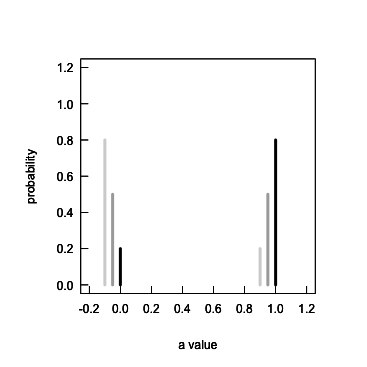
\includegraphics[width=\textwidth]{lectures/day_10_GLMMs/figures/unnamed-chunk-2-1.png} % Add your plot as an image
        \end{column}
    \end{columns}
\end{frame}

\begin{frame}{Binomial distribution}
    \begin{columns}
        \begin{column}{0.5\textwidth}
        Data that can take any discrete values between $0$ and $\infty$ for $n$ trials, with mean $np$ and variance $np(1 - p)$.  
        \begin{align*}
        \text{Binom}(y) &= P(Y = k\; ; n \;p) = \\
        &\binom{n}{k} p^k(1-p)^{n-k}
        \end{align*}
        \end{column}
        \begin{column}{0.5\textwidth}
         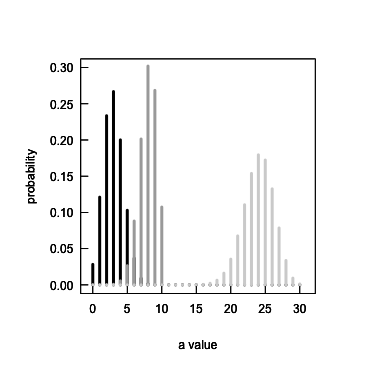
\includegraphics[width=\textwidth]{lectures/day_10_GLMMs/figures/unnamed-chunk-3-1.png} % Add your plot as an image
        \end{column}
    \end{columns}
\end{frame}

\begin{frame}{Poisson distribution}
    \begin{columns}
        \begin{column}{0.5\textwidth}
        Data that can take any discrete values between $0$ and $\infty$, with mean = variance = $\lambda$.  
        \begin{align*}
        \text{Pois}(y) &= P(Y = k\; ; \lambda) = \frac{\lambda^k e^{-\lambda}}{k!}
        \end{align*}
        \end{column}
        \begin{column}{0.5\textwidth}
         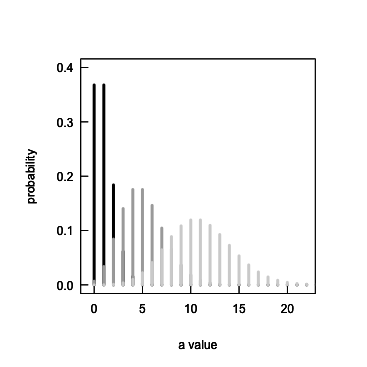
\includegraphics[width=\textwidth]{lectures/day_10_GLMMs/figures/unnamed-chunk-4-1.png} % Add your plot as an image
        \end{column}
    \end{columns}
\end{frame}

\begin{frame}{Mean-Variance Relationships}
    \begin{columns}
        \begin{column}{0.5\textwidth}
            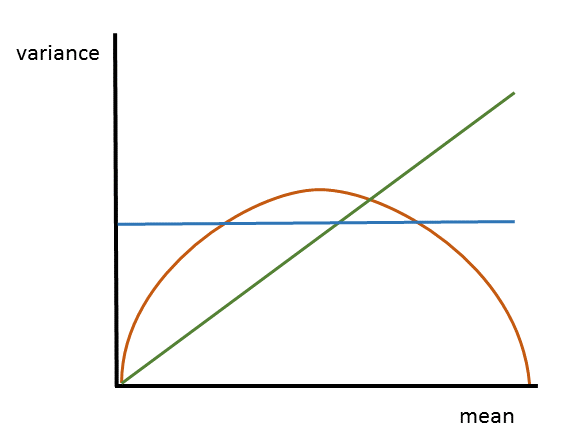
\includegraphics[width=\textwidth]{lectures/day_10_GLMMs/figures/mean-variance.png}
        \end{column}
        \begin{column}{0.5\textwidth}
        \large
            \begin{itemize}
                \item Binomial (orange)
                \item Poisson  (green)
                \item Normal   (blue)
            \end{itemize}
        \end{column}
    \end{columns}
\end{frame}

\begin{frame}{Avoiding Generalised Linear Mixed Models}

\large
\textbf{For use in a glm, remember:}
\begin{itemize}
    \item Ignoring dependencies: simply \textbf{wrong}
    \item Average over groups (Complete pooling)
    \item Use grouping variable as a covariate (no pooling)
\end{itemize}

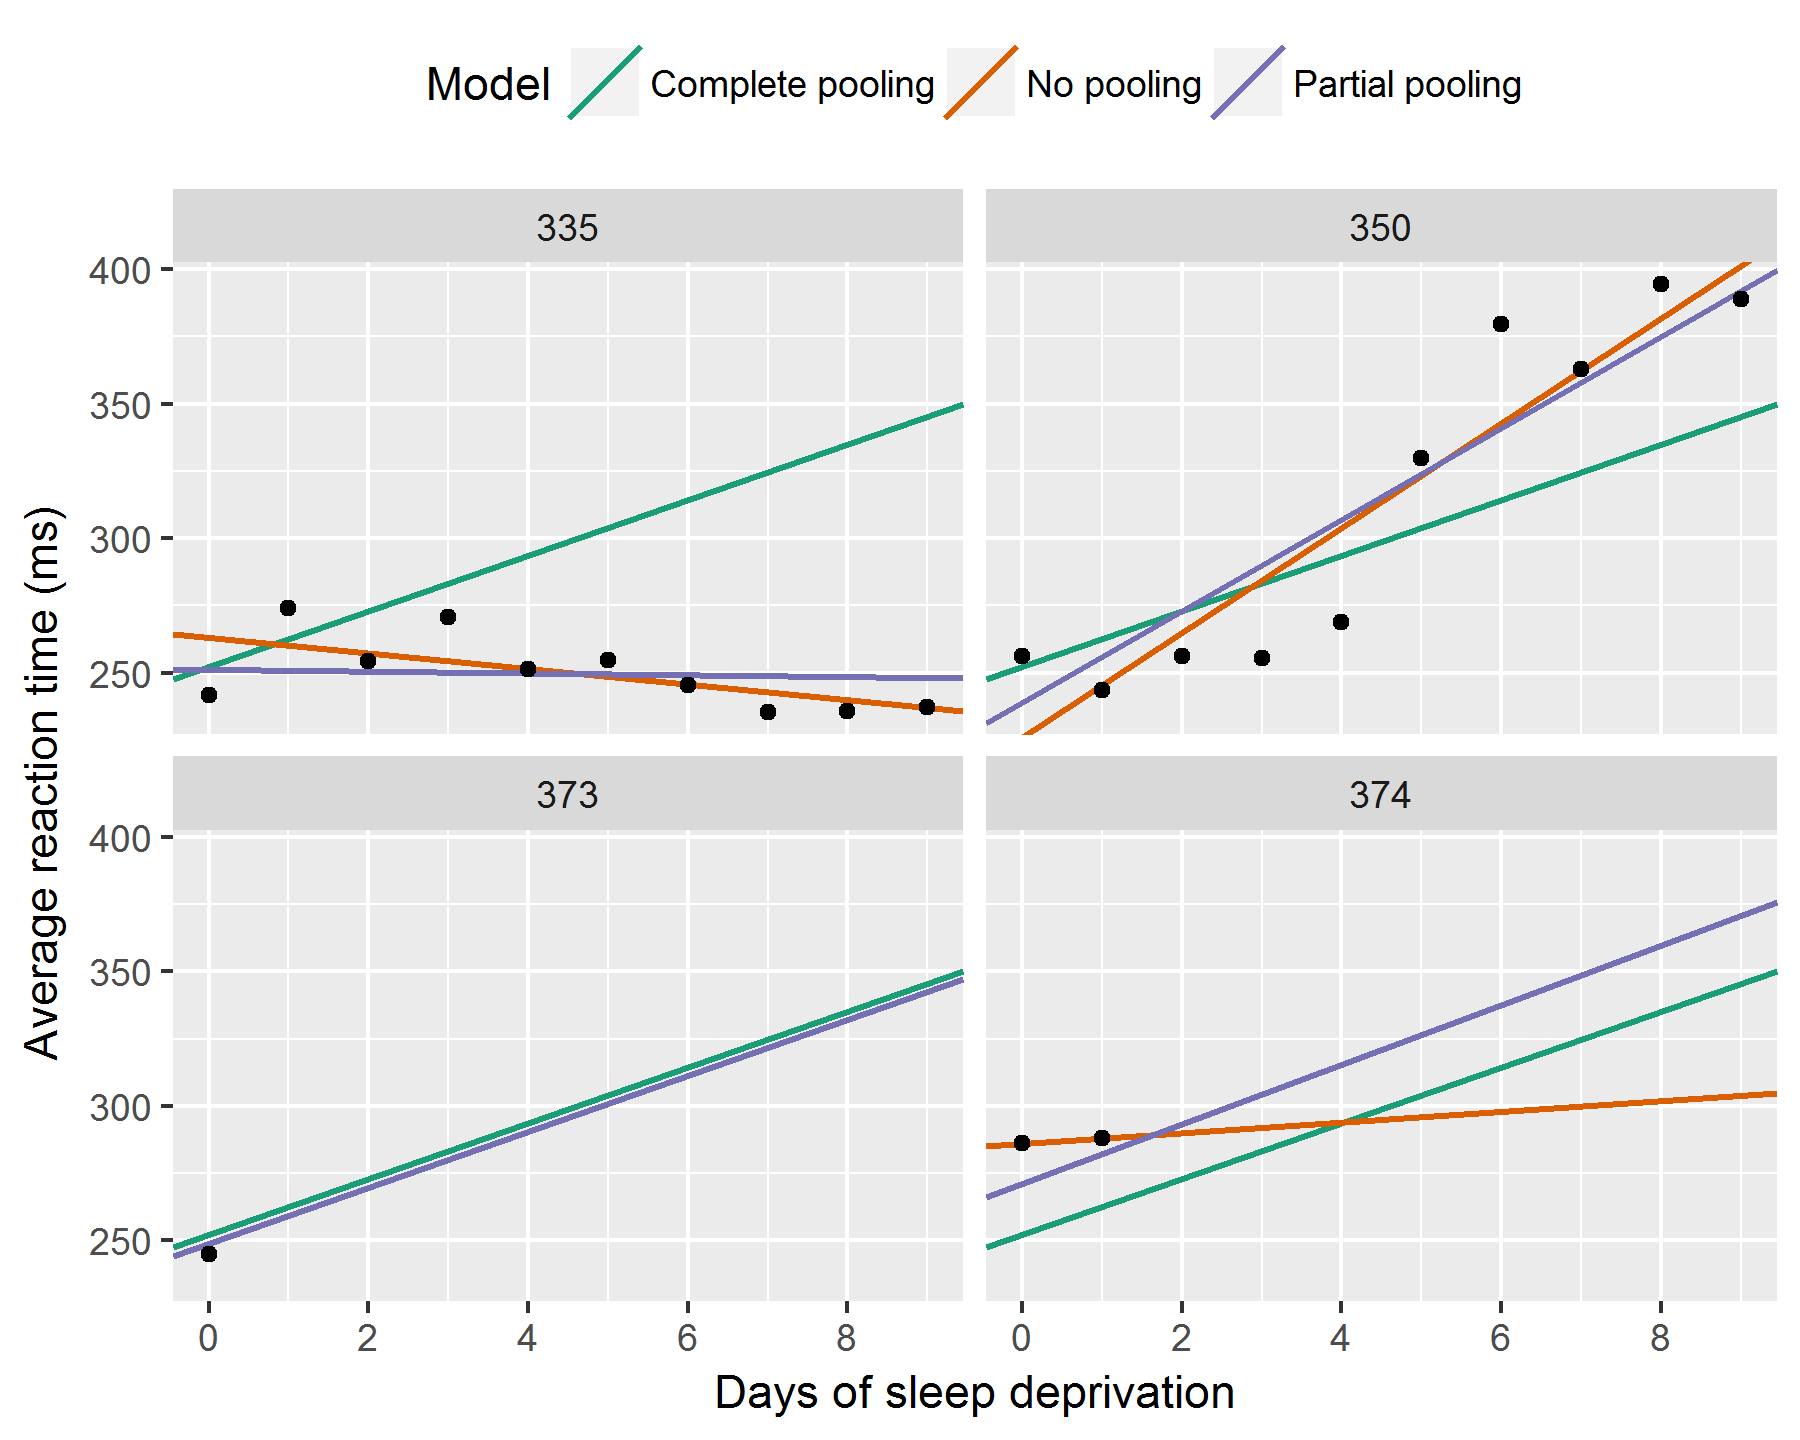
\includegraphics[width=0.6\textwidth]{lectures/day_5_theory_of_mems/figures/zoomed-in-partial-pooling-1.png}
\end{frame}

\begin{frame}[fragile]
\frametitle{Generalised Estimation Equations (GEE)}
\textbf{Analogue to GLS...}

\pause
\begin{itemize}
    \item Generalised Estimation Equations (GEE) allows to explicitly work with the variance-covariance matrix $\mathbf{V_i}$ of the residuals within a group.
    \item GEE lets you define the structure of $\mathbf{V_i}$ and estimate the covariances / correlations.
\end{itemize}
\textbf{In R:}
\scriptsize
\begin{VerbatimIN}[numbers=left,numbersep=6pt]
library(geepack)
# and some other, smaller packages
\end{VerbatimIN}
\end{frame}

\begin{frame}{Marginal Generalised Model}
This again leads to the \textbf{Marginal Generalised Model}
\begin{align*}
    \mathbf{y} &= \mathbf{X} \cdot \mathbf{b} + \mathbf{e}, \quad \epsilon \sim Distr(0, \mathbf{V_i})
\end{align*}
This describes the deterministic part for the average trend in the data while considering the correlation between measurements within a group for \textbf{non-gaussian} data.
\end{frame}

\begin{frame}{Marginal Generalised Model}
    \begin{itemize}
        \item The Marginal Generalized Model is fitted with a \textit{Sandwich Estimator}: there are \textbf{NO} random effects
        \item The Marginal Generalized Model ignores the grouping structure 
    \end{itemize}

    \textit{You won't get among- or within-group variances or group specific (random) intercepts and slopes}
\end{frame}

\begin{frame}{Variance-Covariance Matrix}
All that matters is in the a-priori specified \textit{residual} variance-covariance matrix:
\vspace{0.3cm}

\begin{equation*}
\mathbf{V_i} = \left( \begin{array}{ccccc}
\sigma^2 & c_{12} & c_{13} & c_{14} & c_{15} \\
c_{21} & \sigma^2 & c_{23} & c_{24} & c_{25} \\
c_{31} & c_{32} & \sigma^2 & c_{34} & c_{35} \\
c_{41} & c_{42} & c_{43} & \sigma^2 & c_{45} \\
c_{51} & c_{52} & c_{53} & c_{54} & \sigma^2 \\
\end{array} \right)
\end{equation*}
\vspace{0.3cm}

\textit{Again, zeros in off-diagonals mean that each value has a covariance of zero with all other values being independent}
\end{frame}

\begin{frame}{Correlation Matrix}
Similarly, the correlation matrix:
\vspace{0.3cm}

\begin{equation*}
\mathbf{V_i} = \left( \begin{array}{ccccc}
1 & \rho_{12} & \rho_{13} & \rho_{14} & \rho_{15} \\
\rho_{21} & 1 & \rho_{23} & \rho_{24} & \rho_{25} \\
\rho_{31} & \rho_{32} & 1 & \rho_{34} & \rho_{35} \\
\rho_{41} & \rho_{42} & \rho_{43} & 1 & \rho_{45} \\
\rho_{51} & \rho_{52} & \rho_{53} & \rho_{54} & 1 \\
\end{array} \right)
\end{equation*}
\end{frame}


\begin{frame}[fragile]
\frametitle{Data: Parasites in Red Deer}
    \begin{columns}
        \begin{column}{0.5\textwidth}
        \tiny
            \begin{VerbatimIN}[numbers=left,numbersep=6pt]
head(deers)
            \end{VerbatimIN}
            \begin{VerbatimOUT}[numbers=left,numbersep=6pt]
  Obs Farm Sex Length Ecervi
   2   AL   1  54.18      0
   3   AL   1  46.18      0
   4   AL   1  44.18      1
   5   AL   1  42.18      0
   6   AL   1  38.18      0
   7   AL   1  37.18      1
            \end{VerbatimOUT}
\vspace{0.2cm}

\normalsize
Grouped by Farm\\
Standardised by Length\\
Binary data: parasite yes / no
        \end{column}
        \begin{column}{0.5\textwidth}
        \tiny
        \begin{VerbatimIN}[numbers=left,numbersep=6pt]
hist(deers\$Length)
        \end{VerbatimIN}
        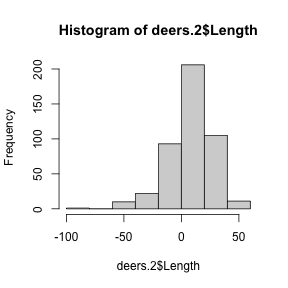
\includegraphics[width=\textwidth]{lectures/day_10_GLMMs/figures/unnamed-chunk-7-1.png}
        \end{column}
    \end{columns}
\end{frame}

\begin{frame}[fragile]
\tiny
    \begin{columns}
        \begin{column}{0.5\textwidth}
            \begin{VerbatimIN}[numbers=left,numbersep=6pt]
plot(deers$Ecervi ~ deers$Length)
            \end{VerbatimIN}
        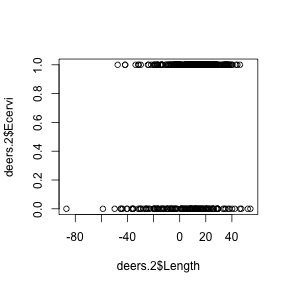
\includegraphics[width=\textwidth]{lectures/day_10_GLMMs/figures/unnamed-chunk-8-1.png}
        \end{column}
        \begin{column}{0.5\textwidth}
            \begin{VerbatimIN}[numbers=left,numbersep=6pt]
xtabs(~Farm, data = deers)
            \end{VerbatimIN}
            \begin{VerbatimOUT}[numbers=left,numbersep=6pt]
Farm
  AL   AU   BA   BE   CB  CRC   HB   LN   
  14   32   22   12   27    1   14   29   
  MAN   MB   MO   NC   NV   PN   QM   RF
  19    17   83   18   0    20   27   12
  RN   RO  SAU   SE   TI   TN VISO   VY 
  16   22    3   15   19    9   13    4 
            \end{VerbatimOUT}
        \vspace{0.2cm}
        \normalsize
Unbalanced group sizes\\
        \end{column}
    \end{columns}
\end{frame}

\begin{frame}[fragile]
    \scriptsize
    \begin{VerbatimIN}[numbers=left,numbersep=6pt]
deers$Farm <- as.factor(deers$Farm) #necessary for grouping !
deers$Sex <- as.factor(deers$Sex)
mod.gee <- geeglm(Ecervi ~ Length*Sex, deers, 
                  family = binomial(link = "logit"), 
                  id = Farm, corstr = "exchangeable")
    \end{VerbatimIN}
    \vspace{0.2cm}
    
    \normalsize
    \textit{id = set to lowest grouping level}\\
    \textit{corstr = set correlation structure}
\end{frame}

\begin{frame}{Unstructured correlation}
Each element above or below the diagonal has to be estimated (here: 10 values)
\vspace{0.3cm}

\begin{equation*}
\mathbf{V_i} = \left( \begin{array}{ccccc}
1 & \rho_{12} & \rho_{13} & \rho_{14} & \rho_{15} \\
\rho_{21} & 1 & \rho_{23} & \rho_{24} & \rho_{25} \\
\rho_{31} & \rho_{32} & 1 & \rho_{34} & \rho_{35} \\
\rho_{41} & \rho_{42} & \rho_{43} & 1 & \rho_{45} \\
\rho_{51} & \rho_{52} & \rho_{53} & \rho_{54} & 1 \\
\end{array} \right)
\end{equation*}

\vspace{0.3cm}

\textit{From the helpfiles: Use unstructured correlation structure only with great care (It may cause R to crash...)}
\end{frame}

\begin{frame}{Exchangeable Correlation}
Similar to the compound symmetry matrix, there is only one element to be estimated:
\vspace{0.3cm}

\begin{equation*}
\mathbf{V_i} = \left( \begin{array}{ccccc}
1 & \rho & \rho & \rho & \rho \\
\rho & 1 & \rho & \rho & \rho \\
\rho & \rho & 1 & \rho & \rho \\
\rho & \rho & \rho & 1 & \rho \\
\rho & \rho & \rho & \rho & 1 \\
\end{array} \right)
\end{equation*}
\vspace{0.3cm}

This is the simplest but sometimes also the least appropriate form.
\end{frame}

\begin{frame}{Temporal Autocorrelation}
Allows the values to be correlated to each other following certain rules as given by the specific autocorrelation function.
\vspace{0.3cm}

The good old \textbf{AR-1} temporal autocorrelation:
\begin{align*}
\epsilon_t &= \rho \cdot \epsilon_{t-1} \\
\text{cor}(\epsilon_s, \epsilon_t) &= 
\begin{cases} 
1 & \text{if } s = t \\
p^{\vert t-s \vert} & \text{if } s \neq t
\end{cases}
\end{align*}
\textit{Decline of relateness with time}
\end{frame}

\begin{frame}
\frametitle{AR-1 temporal autocorrelation}
    \begin{columns}
        \begin{column}{0.5\textwidth}
            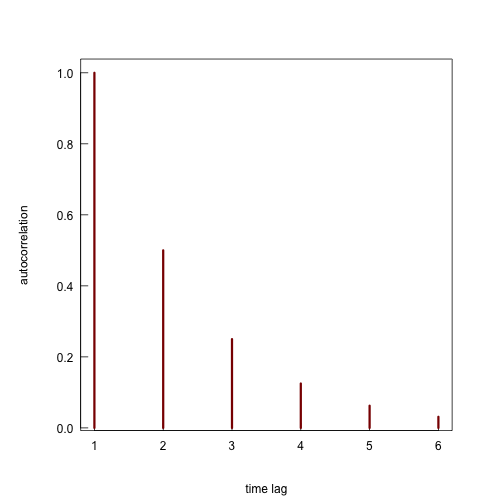
\includegraphics[width=\textwidth]{lectures/day_10_GLMMs/figures/unnamed-chunk-6-1.png}
        \end{column}
        \begin{column}{0.5\textwidth}
        \begin{equation*}
            \mathbf{V_i} = \left( \begin{array}{ccccc}
1 & \rho & \rho^2 & \rho^3 & \rho^4 \\
\rho & 1 & \rho & \rho^2 & \rho^3 \\
\rho^2 & \rho & 1 & \rho & \rho^2 \\
\rho^3 & \rho^2 & \rho & 1 & \rho \\
\rho^4 & \rho^3 & \rho^2 & \rho & 1
        \end{array} \right)
        \end{equation*}
        
        \end{column}
    \end{columns}
\end{frame}

\begin{frame}[fragile]
    \scriptsize
    \begin{VerbatimIN}[numbers=left,numbersep=6pt]
deers$Farm <- as.factor(deers$Farm) #necessary for grouping !
deers$Sex <- as.factor(deers$Sex)
mod.gee <- geeglm(Ecervi ~ Length*Sex, deers, 
                  family = binomial(link = "logit"), 
                  id = Farm, corstr = "exchangeable")
    \end{VerbatimIN}
    \vspace{0.2cm}
    
    \normalsize
    \textit{id = set to lowest grouping level}\\
    \textit{corstr = set correlation structure}
\end{frame}


\begin{frame}[fragile]
    \tiny
    \begin{VerbatimOUT}[numbers=left,numbersep=6pt]
Call:
geeglm(formula = Ecervi ~ Length * Sex, 
       family = binomial(link = "logit"), 
       data = deers, id = Farm, corstr = "exchangeable")

 Coefficients:
            Estimate  Std.err   Wald Pr(>|W|)    
(Intercept) 0.733455 0.273503  7.192  0.00732 ** 
Length      0.030169 0.006943 18.883 1.39e-05 ***
Sex2        0.476311 0.216306  4.849  0.02766 *  
Length:Sex2 0.027280 0.014464  3.557  0.05928 .  
---
Signif. codes:  0 '***' 0.001 '**' 0.01 '*' 0.05 '.' 0.1 ' ' 1

Correlation structure = exchangeable 
Estimated Scale Parameters:

            Estimate Std.err
(Intercept)    1.145  0.3974
  Link = identity 

Estimated Correlation Parameters:
      Estimate Std.err
alpha   0.3305 0.04641
Number of clusters:   24  Maximum cluster size: 209 
    \end{VerbatimOUT}
\end{frame}

%\begin{frame}
%    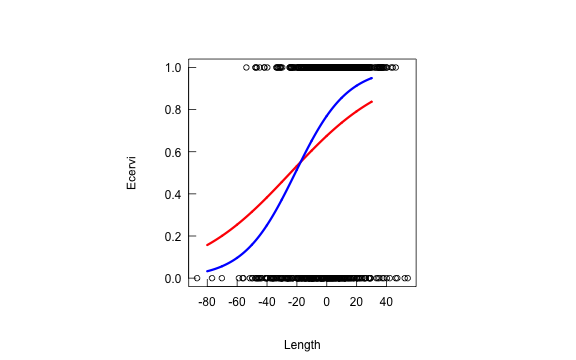
\includegraphics[width=\textwidth]{lectures/day_10_GLMMs/figures/unnamed-chunk-11-1.png}
%\end{frame}


\begin{frame}{The Generalised linear mixed model (GLMM)}
    \large
    \textbf{A GLMM consists of four parts:}
    \begin{itemize}
        \item The fixed-effects part (linear predictor):
        \item[] $\beta_0 + \beta_1 \cdot x$ 
        \item The random-effects part:
        \item[] $u \sim N(0, G)$ 
        \item The stochastic part according to the distribution:
        \item[] $Bern(y), Binom(y), Pois(y)$
        \item The link function
    \end{itemize}
\end{frame}

\begin{frame}{The Link Function}
    It makes sure that the fitting occurs so that the predicted values follow the assumed data distribution:
    \vspace{0.2cm}

    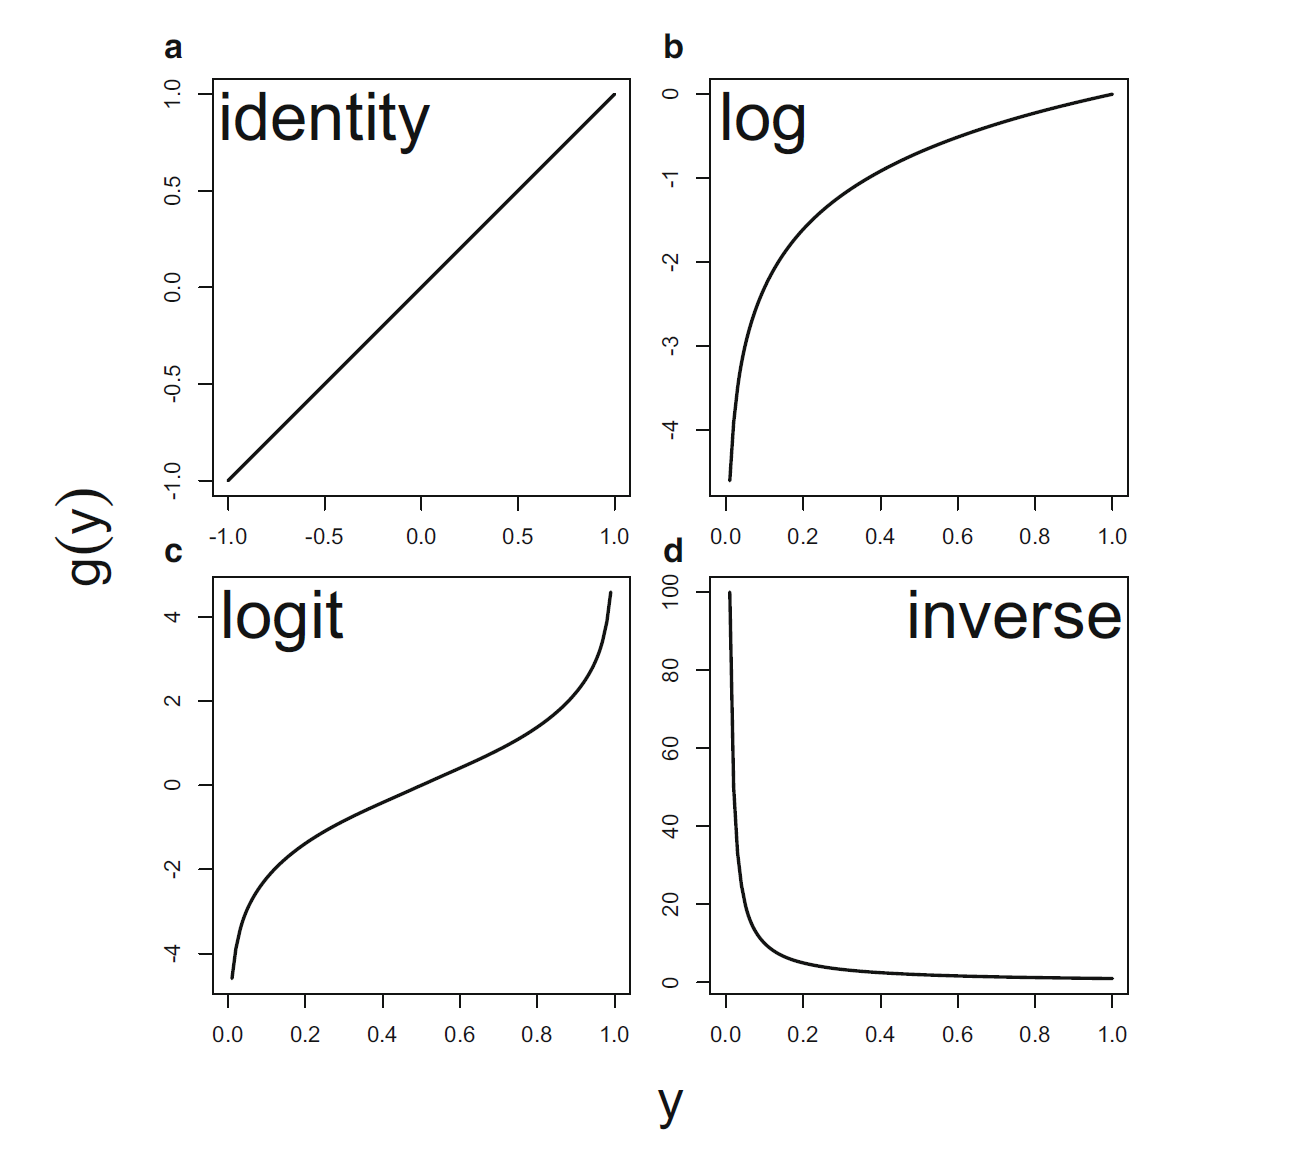
\includegraphics[width=0.6\textwidth]{lectures/day_10_GLMMs/figures/links.png}
    \small (from Dormann 2017)
\end{frame}

\begin{frame}[fragile]
    \tiny
    \begin{VerbatimIN}[numbers=left,numbersep=6pt]
mod.glmm <- glmer(Ecervi ~ Length*Sex + (Length|Farm), deers, 
                  family = binomial(link = "logit"))
summary(mod.glmm)        
    \end{VerbatimIN}
    \begin{VerbatimOUT}[numbers=left,numbersep=6pt]
Generalized linear mixed model fit by maximum likelihood (Laplace
  Approximation) [glmerMod]
 Family: binomial  ( logit )
Formula: Ecervi ~ Length * Sex + (Length | Farm)
   Data: deers

     AIC      BIC   logLik deviance df.resid 
   829.6    862.6   -407.8    815.6      819 
Scaled residuals: 
   Min     1Q Median     3Q    Max 
-6.784 -0.606  0.255  0.514  3.266 
Random effects:
 Groups Name        Variance Std.Dev. Corr
 Farm   (Intercept) 2.388984 1.5456       
        Length      0.000856 0.0293   0.65
Number of obs: 826, groups:  Farm, 24
Fixed effects:
            Estimate Std. Error z value Pr(>|z|)    
(Intercept)   1.0885     0.3661    2.97   0.0029 ** 
Length        0.0430     0.0108    3.98  6.9e-05 ***
Sex2          0.5582     0.2268    2.46   0.0139 *  
Length:Sex2   0.0312     0.0124    2.52   0.0119 *  
---
Signif. codes:  0 '***' 0.001 '**' 0.01 '*' 0.05 '.' 0.1 ' ' 1
Correlation of Fixed Effects:
            (Intr) Length Sex2  
Length       0.326              
Sex2        -0.211  0.107       
Length:Sex2  0.042 -0.434  0.274        
    \end{VerbatimOUT}
\end{frame}

\begin{frame}
    \begin{columns}
        \begin{column}{0.4\textwidth}
            \begin{itemize}
                \item A GEE only gives you the population average (blue)
                \item A GLMM gives you a \textbf{typical} random effects level (red)
                \item A GLMM also gives you the BLUPs (darkred)
            \end{itemize}
        \end{column}
        \begin{column}{0.7\textwidth}
            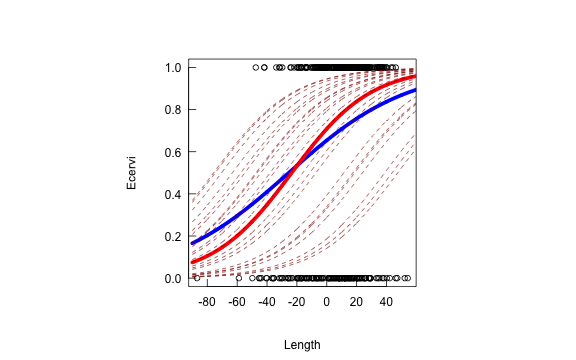
\includegraphics[width=0.999\textwidth]{lectures/day_10_GLMMs/figures/unnamed-chunk-14-1.png}
        \end{column}
    \end{columns}
\end{frame}

\begin{frame}[fragile]
    The assumption for random effects still remains the same:\\
    \[
    \mathbf{u_i} \sim N(0, \mathbf{G})
    \] 
    \vspace{0.2cm}
    
    But the residual variance $\sigma^2$ is missing in the summary:
    \scriptsize
    \begin{VerbatimIN}[numbers=left,numbersep=6pt]
VarCorr(mod.glmm)
    \end{VerbatimIN}
    \begin{VerbatimOUT}[numbers=left,numbersep=6pt]
 Groups Name        Std.Dev. Corr
 Farm   (Intercept) 1.5456       
        Length      0.0293   0.65
    \end{VerbatimOUT}
    \normalsize
    The variance that we know as residual variance is distribution specific, which is fixed on the link scale
\end{frame}


\begin{frame}{Distribution-specific fixed variances on link-scale}

\large These are characteristics of the link-distributions!

\vspace{1cm}
    \large
     \textbf{Binomial on logit-link scale:}\\
     $VAR[Y] = \pi^2 / 3$ 
     \vspace{0.3cm}

     \textbf{Poisson on log-link scale:}\\
     $VAR[Y] = ln(1/(e^{\lambda} + 1))$
     \vspace{0.3cm}

     $\lambda$ is the estimated intercept we get from the estimated model equation on the link-scale
\end{frame}

\begin{frame}[fragile]
\textbf{Repeatability = Intra-Class Correlation}
    \tiny
    \begin{VerbatimIN}[numbers=left,numbersep=6pt]
library(rptR) # can calculate that for you
rpt(Ecervi ~ Length*Sex + (Length|Farm), grname = "Farm", datatype = "Binary", 
    link = c("logit"), data = deers, nboot = 100, adjusted = TRUE)
    \end{VerbatimIN}
    \begin{VerbatimOUT}[numbers=left,numbersep=6pt]
Repeatability estimation using the glmm method and logit link 

Repeatability for Farm
--------------------------------
Link-scale approximation:
R  = 0.383
SE = 0.093
CI = [0.182, 0.529]
P  = 1.57e-40 [LRT]
     NA [Permutation]

Original-scale approximation:
R  = 0.472
SE = 0.167
CI = [0.187, 0.788]
P  = 1.57e-40 [LRT]
     NA [Permutation]
    \end{VerbatimOUT}
    \small
    \textit{Further reading:} \href{https://doi.org/10.1111/j.1469-185X.2010.00141.x}{S. Nakagawa \& H. Schielzeth. “Repeatability for Gaussian and non-Gaussian data: a practical guide for biologists.” Biological Reviews 85 (2010): 935-956.}
\end{frame}

\begin{frame}[fragile]
    Observation-level random effect estimates a second \textbf{variance} term that can absorb extra variance.
    \tiny
    \begin{VerbatimOUT}[numbers=left,numbersep=6pt]
  Obs Farm Sex Length Ecervi
2   2   AL   1  54.18      0
3   3   AL   1  46.18      0
4   4   AL   1  44.18      1
5   5   AL   1  42.18      0
6   6   AL   1  38.18      0
7   7   AL   1  37.18      1
    \end{VerbatimOUT}
    \begin{VerbatimIN}[numbers=left,numbersep=6pt]
mod.glmm.1 <- glmer(Ecervi ~ Length*Sex + (Length|Farm), deers, 
                    family = binomial(link = "logit"))
mod.glmm.2 <- glmer(Ecervi ~ Length*Sex + (Length|Farm) + (1|Obs), deers, 
                    family = binomial(link = "logit"))
    \end{VerbatimIN}
    \begin{columns}
        \begin{column}{0.5\textwidth}
            \begin{VerbatimIN}[numbers=left,numbersep=6pt]
VarCorr(mod.glmm.1)
            \end{VerbatimIN}
            \begin{VerbatimOUT}[numbers=left,numbersep=6pt]
 Groups Name        Std.Dev. Corr
 Farm   (Intercept) 1.5456       
        Length      0.0293   0.65

            \end{VerbatimOUT}
        \end{column}
        \begin{column}{0.5\textwidth}
            \begin{VerbatimIN}[numbers=left,numbersep=6pt]
VarCorr(mod.glmm.2)
            \end{VerbatimIN}
            \begin{VerbatimOUT}[numbers=left,numbersep=6pt]
 Groups Name        Std.Dev. Corr
 Obs    (Intercept) 2.94e-05     
 Farm   (Intercept) 1.55e+00     
        Length      2.93e-02 0.65
            \end{VerbatimOUT}
        \end{column}
    \end{columns}
\end{frame}

\begin{frame}{Diagnostics}
    \Large
    \begin{itemize}
        \item Studentized residuals on the link-scale
        \item over- and underdispersion
        \item zero-inflation and -truncation
    \end{itemize}
\end{frame}

\begin{frame}[fragile]
\frametitle{Diagnostics using DHARMa}
\tiny
    \begin{VerbatimIN}[numbers=left,numbersep=6pt]
library(DHARMa)
res <- simulateResiduals(mod.glmm)
plot(res)    
    \end{VerbatimIN}
    \begin{center}
        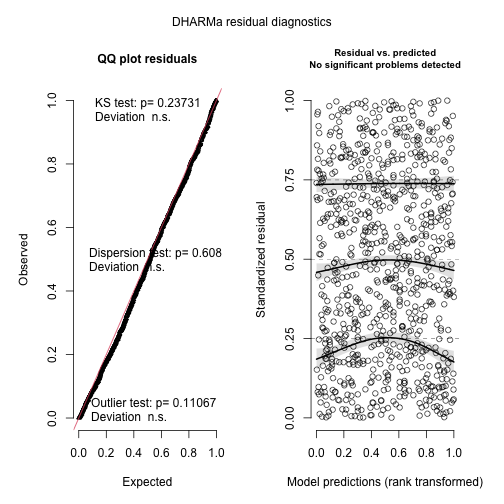
\includegraphics[width=0.5\textwidth]{lectures/day_10_GLMMs/figures/unnamed-chunk-19-1.png}
    \end{center}
\end{frame}

\begin{frame}{Recap Week 11}
    Key concepts covered today:
    \begin{itemize}
        \item GEE vs GLMM
        \item random effects in GLMMs are \textit{normally} distributed
        \item residual variance is distribution-specific
    \end{itemize}
    \vspace{0.2cm}
    
    Today's exercise:\\
    Fitting a GLMM in R
\end{frame}


\begin{frame}{Bloodworm feeding by single convict cichlids }
    \footnotesize Single convict cichlids (fish) were observed for bloodworm ingestions in a laboratory experiment. They were repeatedly fed with bloodworms. Within 2 minutes of the first feeding attempt ("snap"), we waited a maximum of 10 minutes for another snap. If nothing happened, zero was recorded. Fish length (in mm) varied a bit.

    \begin{center}
        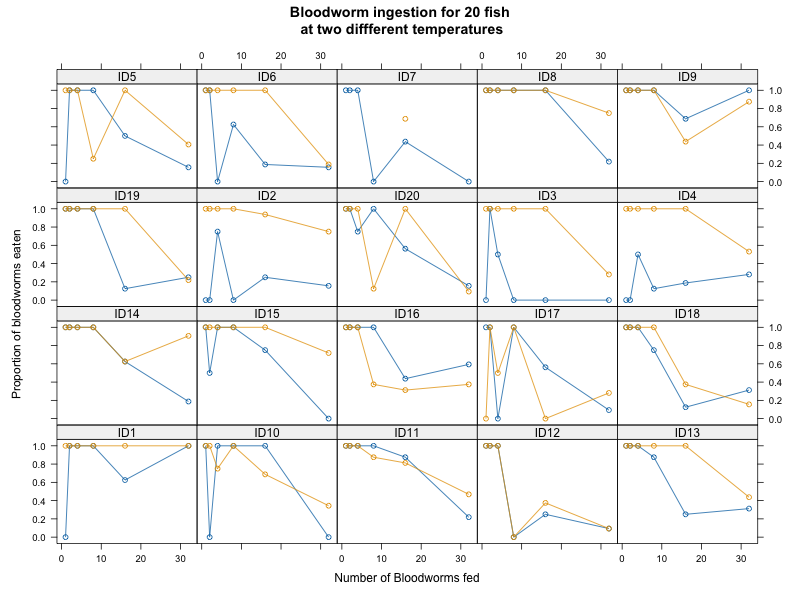
\includegraphics[width=0.8\textwidth]{lectures/day_10_GLMMs/figures/bloodworms.png}
    \end{center}
    
\end{frame}


\begin{frame}[fragile]
\footnotesize The experiment followed a complex blocking design where 20 juvenile convict cichlids were tested over four weeks, with each fish measured 12 times—six times at each of two temperatures (23°C and 29°C). 10 fish were tested per week (Week\_Block), with each food density (1, 2, 4, 8, 16, 32 bloodworms) tested once per week in a randomized order of days (Trial\_Split) from 1 to 6.

    \begin{columns}
        \begin{column}{0.5\textwidth}
        \begin{block}{Randomised days}
{\tiny
            \begin{VerbatimIN}[numbers=left,numbersep=6pt]
xtabs(~Food + Trial_Split, data=ing)
            \end{VerbatimIN}}
\end{block}
            \begin{VerbatimOUT}[numbers=left,numbersep=6pt]
    Trial_Split
Food  1  2  3  4  5  6
  1   4  6  8  8  8  5
  2   8  7  5  6  6  7
  4   8  5  8  7  6  5
  8   8  8  7  7  6  3
  16  7  7  6  7  8  5
  32  4  6  5  4  6 14

            \end{VerbatimOUT}
        \end{column}
        \begin{column}{0.5\textwidth}
            \begin{block}{Blocked Week design}
{\tiny
            \begin{VerbatimIN}[numbers=left,numbersep=6pt]
xtabs(~Food + Week_Block, data=ing)
            \end{VerbatimIN}}
\end{block}
            \begin{VerbatimOUT}[numbers=left,numbersep=6pt]
    Week_Block
Food  a  b  c  d
  1  10 10 10  9
  2  10 10 10  9
  4  10 10 10  9
  8  10 10 10  9
  16 10 10 10 10
  32 10 10 10  9
            \end{VerbatimOUT}
        \end{column}
    \end{columns}
\end{frame}

\end{document}